\chapter{Debugging}
 \label{ch:debugging}

	This chapter explains:
	\begin{itemize}
    \item different types of bugs;
    \item how to use the debugger;
    \item how to use breakpoints and single stepping;
  	\item common errors.
	\end{itemize}

	
  \section{Introduction}
		Debugging is the name given to the job of finding out where the bugs are in a program and then fixing the problem. A bug is an error in a program and, because we are all human, all programs tend to have bugs in them - especially when they are first written. The VB integrated development environment provides a debugger to assist in finding bugs.
		The VB debugger is also a useful tool in helping to understand how variables, assignments, \keyword{If} statements and loops work, because (as we shall see) the debugger can be used to visualize program execution.
As part of the story of where bugs come from, let us trace what happens to a program. There are three stages:
		\begin{enumerate}
			\item	compilation;
			\item linking;
			\item running.
		\end{enumerate}
	We now consider these in turn.


		\subsection*{Compilation}
			As you type in a program, the VB development environment carries out comprehensive checks, exposing many errors that might otherwise persist. These errors are shown underlined as soon as you type the program statements. These errors are termed compilation errors. A common example is an undeclared variable.
			
			It is important to ensure that the options \ui{Explicit} and \ui{Strict} are switched on. Go to \ui{Tools | Options | Project and Solutions | VB defaults} and switch these options \ui{On}. These ensure that the greatest possible error checking is brought into action. The first option ensures that the compiler checks that all variables are declared. The second option makes the compiler check that all data conversions are carried out explicitly. For example, in the following code extract:
			\begin{lstlisting}
Dim age As Integer
age = CInt(TextBox1.Text)
			\end{lstlisting}
			the string in the text box is explicitly converted into an integer value.
			
			When all the errors have been corrected, the program will compile ‘cleanly’ and it will execute, even though it may not do exactly what you want.


		\subsection*{Linking}
			All programs make use of library methods and some make use of programmer-written classes. These classes are linked only when the class is called, when the program is running. But the integrated development environment checks a program as soon as it is typed in, to ensure that all the methods that are called do exist and that the parameters match in number and type. Again, any errors are shown underlined as soon as you type the program statements.


		\subsection*{Running}
			A program runs, but it is most unusual for it to work first time as expected. In fact it is usual for the program to fail in some way or behave in a way other than was intended. Some errors are detected automatically and the programmer is notified – like an attempt to divide \keyword{Integer} quantities by zero. Others are subtler and simply give rise to unexpected behaviour. You have a bug in the program – or more likely many bugs! So you have to carry out some debugging.
			
			Later on in this chapter we give examples of common errors that arise in VB programming.
			
			The term ‘bug’ originated in the days of valve computers, when (the story goes) a large insect became lodged in the circuitry of an early computer, causing it to malfunction. Hence the term ‘bug’ and the term ‘debugging’.

			The problem with debugging is that the symptoms of a bug are usually rather uninformative. So we have to resort to detective work to find the cause. It’s like being a doctor: there is a symptom, you have find the cause, then you have to fix the problem.
			
			Once the more obvious faults in a program have been eliminated, it is usual to start carrying out some systematic testing. Testing is the repeated running of a program with a variety of data as input and is discussed in \Cref{ch:testing}. The aim of testing is to convince the world that the program works properly. But normally testing reveals the existence of more bugs. Then it is time to do some debugging. So testing and debugging go hand-in-hand.
			
			Many programmers like debugging; they see it as exciting – like watching a mystery thriller in which the villain is revealed only at the last moment. Certainly, along with testing, debugging often takes a long time. Do not be worried that debugging takes you some time – this is normal!

			
	\section{Using the debugger}
		A program runs but behaves unexpectedly. How do we find the source of the problem? Most programs display something on the screen, but otherwise what they do is invisible. We need something like X-ray specs to gain some insight into how the program is behaving. This is the key to successful debugging – getting additional information about the running program.
		
		The VB integrated development environment provides a \emph{debugger}. A debugger is a program that helps you debug your program. It runs alongside your program, allowing the progress of the program to be inspected. It provides several facilities, including single stepping and breakpoints.
		

		\subsection*{Breakpoints}
			Using the debugger, the programmer can place a \emph{breakpoint} in the program. A breakpoint is a place in the program where execution stops. A breakpoint is inserted as follows:
			\begin{enumerate}
				\item	Click on the vertical grey bar to the left side of a line in the text of the program (\Vref{fig:debugging_breakpoint}) (the line is highlighted in brown and a brown circle is shown on the grey bar).
				\item	Start the program as usual.
			\end{enumerate}
			\begin{figure}[bth]
				\centering
				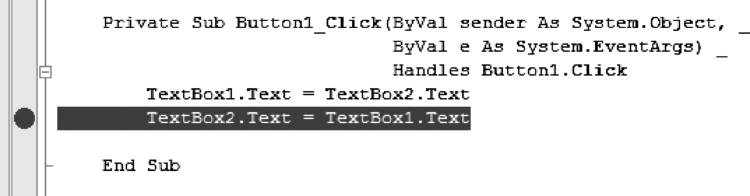
\includegraphics[width=12cm]{debugging_breakpoint}
				\caption{Placing a breakpoint.}
				\label{fig:debugging_breakpoint}
			\end{figure}
			When the breakpoint is reached, the program pauses as it is just about to execute the line highlighted in yellow. A yellow pointer is shown superimposed on the brown circle. You can then position the cursor over the name of a variable or a property and see its value displayed. Any discrepancy between what the value actually is and what it should be provides valuable information for debugging.
			
			Instead of displaying values by placing the cursor over the name, a watch window can be created. This is a separate window that displays the values of selected variables. Right-clicking on a variable name displays a menu, part of which is shown in \Vref{fig:debugging_variable_menu}.
			\begin{figure}[bth]
				\centering
				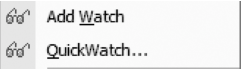
\includegraphics[width=5cm]{debugging_variable_menu}
				\caption{Part of the menu obtained by right-clicking on a variable name.}
				\label{fig:debugging_variable_menu}
			\end{figure}
			
			Selecting \ui{Add Watch} creates the watch window, showing the variable name and its value (\Vref{fig:debugging_watch_window}). Any number of variables can be added to this watch window, so that their values can be continuously monitored.
			\begin{figure}[bth]
				\centering
				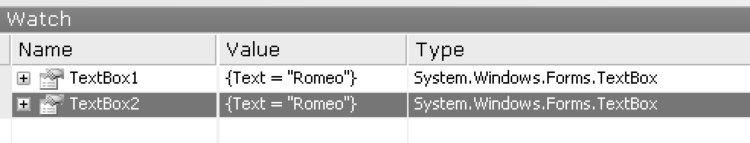
\includegraphics[width=12cm]{debugging_watch_window}
				\caption{The \ui{Watch} window.}
				\label{fig:debugging_watch_window}
			\end{figure}
			
			Once information has been obtained, an individual breakpoint can be removed by clicking on the brown dot to the left of the line.
			
			Multiple breakpoints can be inserted into a program. Once a breakpoint is reached, clicking on \ui{Continue} on the \ui{Debug} menu resumes execution of the program until it either ends or reaches the next breakpoint.
			
			To find bugs quickly, the trick is to choose the best points in the program for breakpoints. Generally, good points to choose are:
			\begin{itemize}
	      \item At the start of a method, to check that the parameters are OK.
  	    \item Immediately after a method has been called (to check that the method has done its work correctly) or right at the end of the method (for the same reason).
			\end{itemize}


		\subsection*{Single stepping}
			The debugger also allows us to execute a program one line at a time; this is called \emph{single stepping}. This is achieved by selecting \ui{Step Into} from the \ui{Debug} menu, or more conveniently using a function key. (The number of this function key depends on your setup. Look at the Debug menu, \Vref{fig:debugging_debug_menu}, to see which it is.) The program executes a line and pauses before the line that is highlighted. Any difference between the expected path and the actual path of execution gives useful information about the cause of the bug. At any time we can place the cursor over a variable name and observe its value. Alternatively, we can set up a watch window as explained above. Again, any difference between the expected value and the actual value gives useful information.
			\begin{figure}[bth]
				\centering
				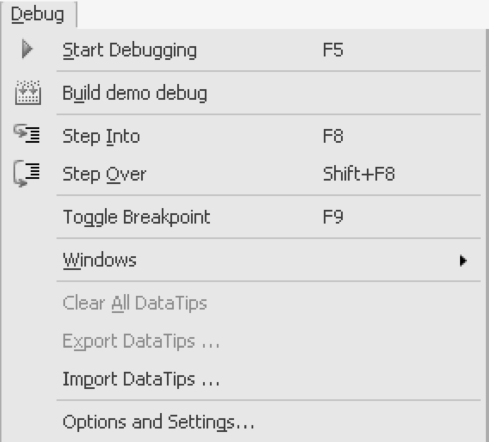
\includegraphics[width=5cm]{debugging_debug_menu}
				\caption{The \ui{Debug} menu.}
				\label{fig:debugging_debug_menu}
			\end{figure}

			
			It is easy to have a lot of fun with a debugger, but the downside can be using a lot of time. A productive way to use a debugger is as follows:
			\begin{enumerate}
				\item From the symptoms of the bug, make a hypothesis about where the bug lies. You may be able to predict that the error lies within any of two or three methods.
				\item Place breakpoints at the entry and exit of the methods under suspicion.
				\item	Run the program. When the program stops at the entry to a method, inspect the values of the parameters. At the exit, inspect the value of the return value and the values of significant instance variables. Thus identify the method within which the bug lies.
				\item Run the program again, stopping at the entry to the erroneous method. Single step through this method until you see the discrepancy between expectation and reality. You have found the bug.
			\end{enumerate}


	\section{Case study in debugging}
	The program (\Vref{fig:debugging_romeo_juliet_screen}) illustrates the love between Romeo and Juliet. A button is provided to swap the names in the two text boxes. But the code, as written, simply displays the same name in each box. The erroneous code is:
			\begin{figure}[bth]
				\centering
				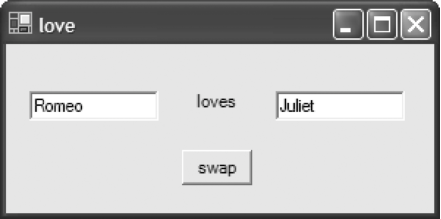
\includegraphics[width=5cm]{debugging_romeo_juliet_screen}
				\caption{The Rome and Juliet program.}
				\label{fig:debugging_romeo_juliet_screen}
			\end{figure}
		\begin{lstlisting}
Private Sub Button1_Click(sender As System.Object,
		e As System.EventArgs)
		Handles Button1.Click
	LeftTextBox.Text = RightTextBox.Text
	RightTextBox.Text = LeftTextBox.Text
End Sub
		\end{lstlisting}
		There is only one method in this program, so the source of the problem must be within this method. We place a breakpoint at the beginning of the method and then single step through the statements, placing the cursor over the two variables (the text box values) to display their values. Alternatively we create a watch window, as described above. It becomes immediately clear that the value of \keyword{LeftTextBox.Text} has been overwritten and therefore lost. We have made a classic mistake – which we can rectify by storing this value in a temporary variable as follows:
		\begin{lstlisting}
Private Sub Button1_Click(sender As System.Object,
		e As System.EventArgs)
		Handles Button1.Click
	Dim temp As String
	temp = LeftTextBox.Text
	LeftTextBox.Text = RightTextBox.Text
	RightTextBox.Text = temp
End Sub
		\end{lstlisting}


	\section{Common errors}
		Certain errors are commonly made by VB programmers. We list some of them below. It’s worthwhile checking any suspect program for these errors.


		\subsection*{Compilation errors}
			The VB development environment carries out a lot of checking on a program as you type in the program and displays a curvy blue line underneath anything it finds that is a problem. These are termed compilation or syntax errors. You can get a brief explanation of the error by positioning the cursor over the curvy line. This is part of trying to ensure that VB programs are robust. An error caught at compile-time is easily fixed, but any errors left undetected until run-time may take a lot of debugging. So although compile-time errors can be annoying, they are good value.

			Here are some areas which often cause compilation errors:
		

			\subsubsection*{Variable names}
				All variables should be declared and then spelled consistently. It is tempting on occasion to use a keyword as a variable name (for example, the word Error is a keyword).


			\subsubsection*{Method and property names}
				It is not unusual to:
				\begin{itemize}
					\item omit an \keyword{Imports} statement;
    		  \item misspell a method or property name;
		      \item get the parameters for a method wrong.
				\end{itemize}

				
			\subsubsection*{Conversions}
				If you write:
				\begin{lstlisting}
TextBox1.Text = 23
				\end{lstlisting}
				you will get an error message (code underlined with a wiggly blue line) to say that an implicit conversion from string to number is not allowed. This needs to be done like this:
				\begin{lstlisting}
TextBox1.Text = CStr(23)
				\end{lstlisting}
				A similar error can occur when a number is input via a text box:
				\begin{lstlisting}
Dim number As Integer
number = TextBox1.Text
				\end{lstlisting}
				This causes a compilation error message saying that the text needs to be explicitly converted to a number. To remedy this problem, the conversion can be accomplished as follows:
				\begin{lstlisting}
number = CInt(TextBox1.Text)
			\end{lstlisting}

			
		\subsection*{Run-time errors}
			Run-time errors are errors that occur as the program is running, but are detected by the run-time system. Again this is part of the measures designed to ensure that programs are robust – preventing a program that has gone wrong acting like a bull in a china shop. Run-time errors lead to an error message being displayed and the program being stopped.


			\subsubsection*{Arithmetic exceptions}
				If a program attempts to divide by zero, the program will stop and an error message is displayed. It is fairly easy to let this happen inadvertently, for example in a program that contains this fragment:
				\begin{lstlisting}
Dim a, b, c As Integer
b = 1
c = CInt(TextBox1.Text)
a = b / c
				\end{lstlisting}
				If the user enters the number zero into the text box, an attempt is made to divide by zero, the program is stopped and a message box is displayed (\Vref{fig:debugging_overflow_exception}). The line of VB that caused the error is highlighted in yellow.
				\begin{figure}[bth]
					\centering
					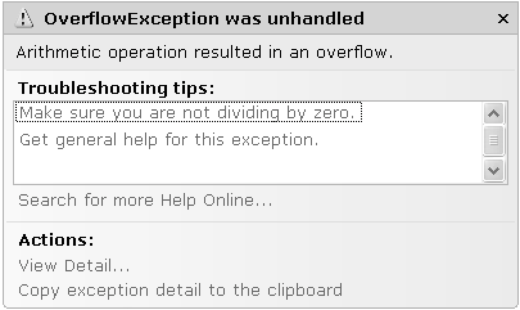
\includegraphics[width=8cm]{debugging_overflow_exception}
					\caption{Division by zero.}
					\label{fig:debugging_overflow_exception}
				\end{figure}

				
				The message box tells us fairly clearly what has happened – a calculation was attempted, but overflow occurred. Clicking on \ui{Continue} causes the program to continue execution. Clicking on \ui{Break} allows us to inspect the values of variables.
				
				A remedy for this situation is to write code to check the value of c before the division takes place.


			\subsubsection*{Array indices}
				The topic of arrays is something that we will not explain until \Cref{ch:arrays} However, we have included here for completeness a common error that arises when arrays are used. If an array is declared as:
				\begin{lstlisting}
Dim table(10) As Integer
Dim index As Integer
For index = 0 To 11 ‘warning, erroneous	
	table(index) = 0
Next
				\end{lstlisting}
				This places a zero in all of the elements of the array \keyword{table}, but then goes on to try to place a zero in index value 11. This is beyond the end of the array, so the program fails and a message box (\Vref{fig:debugging_index_exception}) is displayed. The VB statement that caused the error is highlighted. The message is fairly clear in telling us that the index was out of range.
				\begin{figure}[bth]
					\centering
					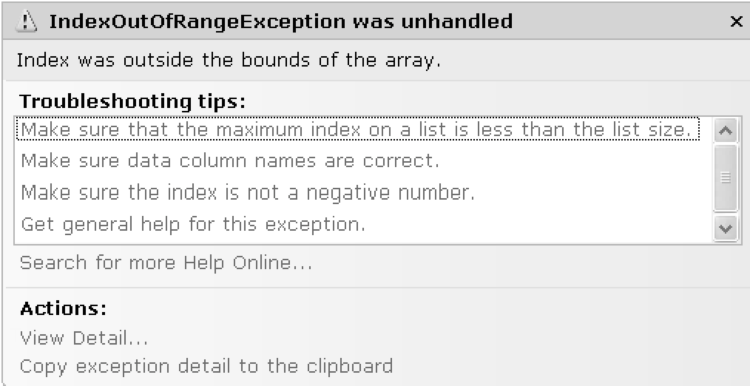
\includegraphics[width=8cm]{debugging_index_exception}
					\caption{Array index out of range.}
					\label{fig:debugging_index_exception}
				\end{figure}
				
				The remedy for this situation is to correct the design flaw in the code.


			\subsubsection*{Using a non-existent object}
			In earlier chapters we saw how to declare an object as an instance of a class. For example we can declare a variable \keyword{ageGuesser} as a variable of the class \keyword{Random}:
				\begin{lstlisting}
Dim ageGuesser As Random
				\end{lstlisting}
				If we now try to use the variable \keyword{ageGuesser} by calling the method \keyword{Next} as follows:
				\begin{lstlisting}
Dim age As Integer
age = ageGuesser.Next(5, 110)
				\end{lstlisting}
				the program will fail and a message box (\Vref{fig:debugging_null_exception}) is displayed.
				\begin{figure}[bth]
					\centering
					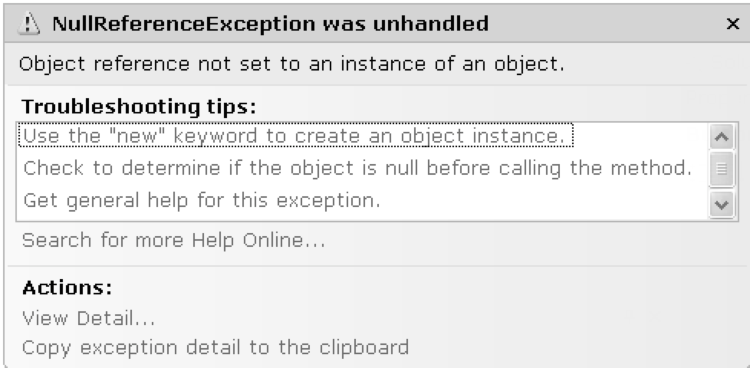
\includegraphics[width=8cm]{debugging_null_exception}
					\caption{Attempt to use a non-existing object.}
					\label{fig:debugging_null_exception}
				\end{figure}

				
				We have attempted to use an object that has not been created. What was missing was an instruction to create an instance of the \keyword{Random} class, such as:
				\begin{lstlisting}
ageGuesser = New Random()
				\end{lstlisting}
				
		
		\subsection*{Logic errors}
			Logic errors are the hardest to find, because they depend on the way that the individual program works. Therefore there is no automatic way of detecting such errors. Two types of error are, however, common.
			
			Initialization means giving a variable an initial value, and it is easy to fail to initialize a variable appropriately. In VB, all variables are automatically initialized to some definite value – for example, \keyword{Integer} values are initialized to zero automatically – but this may not be the required value.
			
			It is all too easy to fail to provide handling for an event (a click on a button, for example). This can happen when you change the name of a component such as a button, but forget to match the change of name in the \keyword{Handles} part of the event handler method.
			

	\section{Programming pitfalls}
		Ensure that the \keyword{Explicit} and \keyword{Strict} options are always switched on. This reduces errors by ensuring that the compiler does its utmost to check the program.


	\section{New IDE facilities}
		To insert or remove a breakpoint, click on the grey bar at the left of the line. The \ui{Debug} menu provides the facility to single step through a program.


	\section{Summary}
		\begin{itemize}
      \item Debugging is finding errors (bugs) in a program and fixing them.
      \item The VB integrated development environment provides a ‘debugger’ program.
      \item A breakpoint is a place where the program temporarily stops.
      \item Single stepping is watching the execution flow through the program.
      \item The values of variables can be displayed at breakpoints or during single stepping.
		\end{itemize}


	\section{Exercise}
		
		\begin{EXE}
			\item	Using a program that you have already written, practise using the debugger. Place breakpoints within the program and run it. Then single step through the program, placing the cursor over variable names so as to display their values.
		\end{EXE}
